% !TeX program = lualatex

\documentclass[12pt]{report}
\usepackage[table,xcdraw]{xcolor}
\usepackage[Glenn]{fncychap}
\usepackage[T1]{fontenc}
\usepackage[francais]{babel}
\usepackage{fontspec}
\usepackage{wrapfig}
\usepackage{graphicx}
\usepackage[a4paper, width=175mm, top=25mm, bottom=25mm]{geometry}
\usepackage{parskip}
\usepackage{enumitem}
\usepackage{titlesec}
\usepackage{listings}
\usepackage{float}
\usepackage[final]{pdfpages}
\usepackage{tocbibind}
\usepackage{tocloft}
\usepackage{xpatch}
\usepackage{amsmath}
\usepackage{amsthm}
\usepackage{amsfonts}
\usepackage{graphics}
\usepackage{framed}
\usepackage{multirow}
\usepackage{graphicx}
\usepackage[utf8x]{inputenc}
\setcounter{secnumdepth}{3} 
\usepackage{mathtools}
\usepackage{amsmath}
\usepackage{tabularx}
\usepackage[ruled,french,onelanguage]{algorithm2e}
\usepackage{tikz}
\usepackage{multirow}
\usepackage[noend]{algpseudocode}
\usepackage{tabularx}  % for tabularx
% to make cells in table have decent spacing
\usepackage{diagbox}
\usetikzlibrary{arrows, positioning, automata}

\usepackage{array}
\newcolumntype{L}[1]{>{\raggedright\let\newline\\\arraybackslash\hspace{0pt}}m{#1}}
\newcolumntype{C}[1]{>{\centering\let\newline\\\arraybackslash\hspace{0pt}}m{#1}}
\newcolumntype{R}[1]{>{\raggedleft\let\newline\\\arraybackslash\hspace{0pt}}m{#1}}


\begin{document}
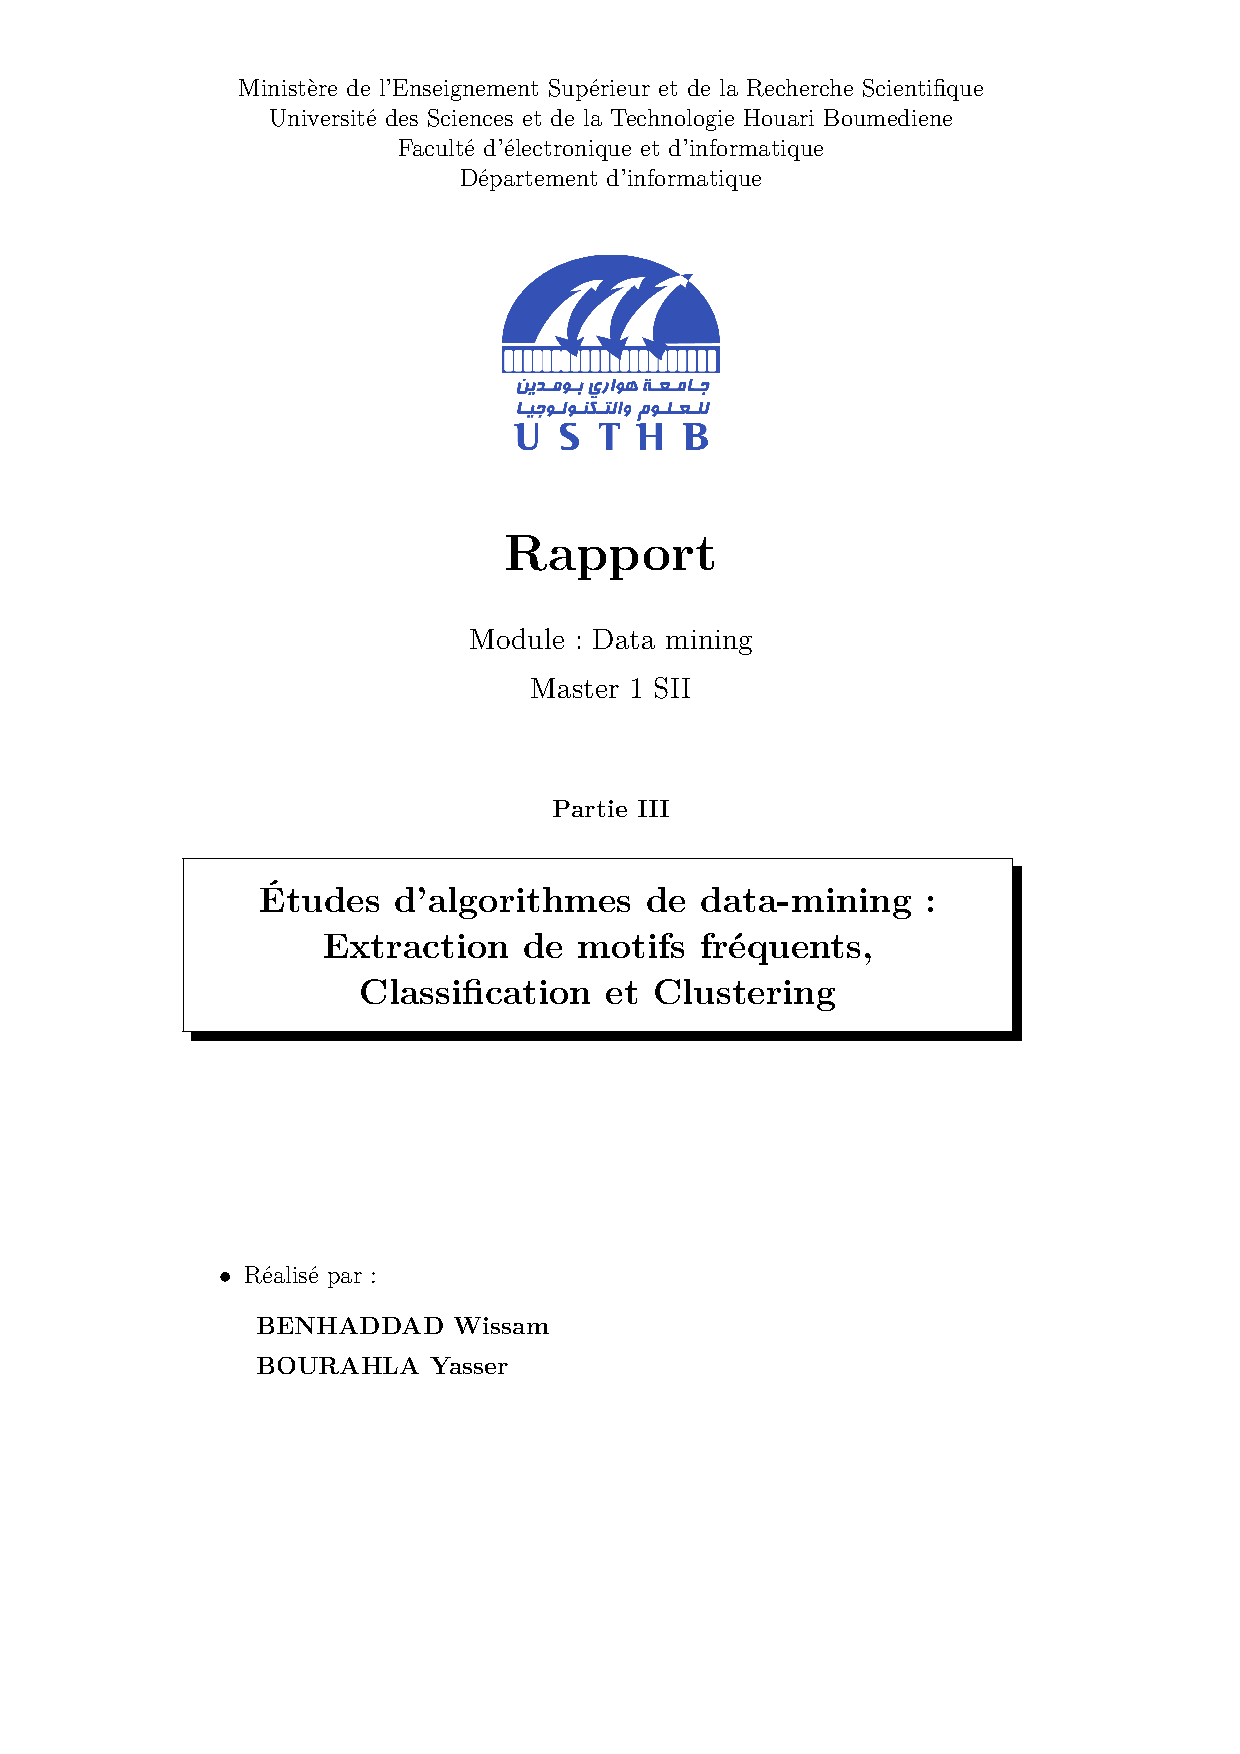
\includepdf[pages=1]{Page_garde.pdf} 
\tableofcontents

\pagenumbering{arabic}
\newpage


\chapter{Introduction et problématique}



\setlist[itemize]{label=\textbullet}
\chapter{Extraction de motifs fréquents à l'aide de l'algorithme Apriori}\label{apriori}
	\section{Introduction}
		\paragraph{}
		Souvent confronté à un ensemble de données qui n'ont vraisemblablement pas une régularité ou des sous structures qui se répètent suivant un certain motif, Une des tâches la plus répandue dans le domaine du Data-Mining est l'extraction de ces dits \textbf{Motifs fréquents}.
		\par 
		De façon informelle, un motifs fréquent peut être un item(objet, article ...) une sous-séquences d'items, une sous-structure(sous-graphe, sous-ensemble ...) qui se répète un certain nombre minimum de fois dans la base de données, ce qui lui vaut le nom de motifs \textbf{fréquent}\cite{Han}.
		\par 
		Dans ce qui suit nous allons voir deux algorithmes capables tout deux d'extraire de tels motifs, l'algorithme \textbf{Apriori} \cite{Agrawal:1994:FAM:645920.672836} et l'algorithme FP-Growth \cite{Hanfp}
		
	\section{Définitions}
		\paragraph{}
		Avant d'introduire les deux algorithmes, il faut d'abord définir quelques concepts qui sont intrinsèquement reliés au déroulement de ces deux derniers:
		\subsection*{Items}
			\paragraph{}
			Un item $I_i$ est généralement un attribut associé à un dataset(Taille,Poids,Catégorie...), cet item a un domaine de définition $D_{I_i}$.
		
		\subsection*{Transaction}\label{transaction}
			\paragraph{}
			Une transaction $T_i$ est généralement une instance du dataset, elle se présente comme un ensemble d'items aux quels une valeur à été attribué : 
			$T_i = \lbrace t_1,t_2,...,t_n\rbrace$, on lui associe un identifiant unique $id_{D_i}$.
		
		\subsection*{Support}
			\paragraph{}
			Un support $S$ est un indicateur(une mesure) de combien de fois un ensemble d'item $X$ apparaît dans un dataset $T$, il est définie comme le nombre de transactions $t$ qui contiennent l'itemset $X$ : 
		
			\begin{equation*}
				Support(X) = \frac{|t \in T ; X \subseteq t|}{|T|}
			\end{equation*}
		
	\section{Algorithme}
		\paragraph{}
		Apriori est un algorithme proposé par Agrawal et Srikant en 1994 dans \cite{Agrawal:1994:FAM:645920.672836}, son but est l'extraction de motifs fréquents dans une base de données de transactions \ref{transaction}.
		\par Apriori construit les ensembles d'items candidats à partir d'un ensemble d'items singletons en générant à chaque itérations une extension de ces derniers en ajoutant un item à la fois tout en testant la condition de support minimum ainsi que la condition de sous-motifs fréquent \footnote{Si $M$ est un motif fréquent alors $\forall m_i \in M $ $m_i$ est aussi un item fréquent} pour permettre l'élimination plus rapide des itemsets candidats, l'algorithme s'arrête quand aucune extension ne peut être générée, le pseudo code est le suivant :
		
	
		\begin{algorithm}[H]
			\caption{Apriori}
			\SetKwInOut{Input}{Entrée}\SetKwInOut{Output}{Sortie}
			\SetKwFunction{gen}{GenererCandidats}
			\SetKwFunction{contains}{Contient}
			
			\Input{(T : Ensemble des transactions , $Sup_{min}$ : entier )}
			\Output{(L : Ensemble des items fréquents)}
			\textbf{Var :} \\
			$C_k : $ Itemset des candidats de taille $K$
			$L_k : $ Itemset des items les plus fréquents de taille $K$
			
			
			\Begin
			{
				$L_1$ \gets $\lbrace items les plus fréquent \rbrace$ ;\\
				\For{($k \gets $ ; $L_k \neq \emptyset $ ; $k \gets k+1$)}
				{
					$L_{k+1} \gets $ \gen{$L_k$};\\
					\ForEach{transaction $t \in T$ }
					{
						\For{candidat $c \in C_{k+1}$}
						{
							\If{\contains{$t$,$c$}}
							{
								$compteur[c] \gets compteur[c]+1$
							}
						}
						
					}
					$L_{k+1} \gets \lbrace 	c | c \in C_{k+1} \land compteur[c] \geq Sup_{min}\rbrace$ 	
				}
				
			}
			\KwRet{$\bigcup\limits_{m} L_m ; m = 0,k $}
		\end{algorithm}
	\section{Implémentation}
		
			\paragraph{}
			Le module \textbf{Apriori} se décompose principalement de trois parties : 
			\begin{itemize}
				\item \textbf{Chargement des données} : la phase où l'on récupère une instance d'un jeu de donnée à travers un fichier d'extension \textbf{.arff} qui contiendra les données et les méta-donnés associée (Nombre d'attributs, leurs types, valeurs manquantes ...), les chargeant en mémoire pour le traitement suivant.
				\item  \textbf{Traitement sur les données} : c'est le coeur du système, c'est ici que l'algorithme va extraire les connaissances souhaitées en appliquant l'algorithme mentionné dans (REFEREEEEEEEEEENCE TO APRIORI), les détails de l'implémentation seons mentionner 
			\end{itemize}
			\par 
			Pour se faire nous avons implémenté 3 classes \textbf{Java} qui effectuent chacune un travail bien précis, communiquant son résultat à une classe. Un schémas récapitulatif est présenté ici suivi d'une explication sur le fonctionnement de chacune des classes(avec les structures de données qu'elles manipulent)
			
			\begin{figure}[H]
				\centering
				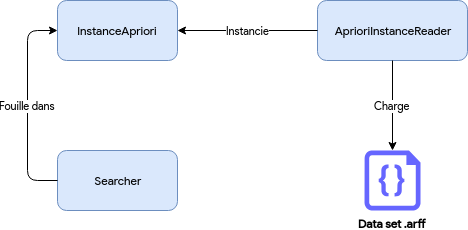
\includegraphics[width=0.75\linewidth]{apriori/images/apriori_schema.png}
			\end{figure}
		
			\subsection{InstanceApriori : } c'est la classe qui va contenir l'ensemble des transactions ainsi que les méthodes manipulant, les attributs sont les suivants : \\
			\begin{figure}[H]
				\centering
				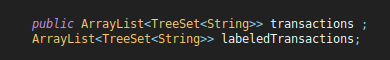
\includegraphics[width=0.75\linewidth]{apriori/images/data_structs/instance/properties.png}
			\end{figure}
			\par 
			Le choix de la structure \textbf{TreeSet} garantie un accès, ajout et suppression d'une entrée en $O(log(n))$, les transactions seront donc représenté comme un vecteur d'ensemble de chaînes de caractères. la différence entre les deux attributs(attribut au sens Orienté-Objet) est que le 2e contient des ensemble de transactions de la forme \textbf{<attribut:valeur\_attribut>}, c'est cette représentation qui sera choisie pour le traitement, l'autre sera utilisé pour l'affichage car il ne dispose pas de l'information sur l'attribut
			\par Pour ce qui en est des méthodes utilisées : 
			\begin{figure}[H]
				\centering
				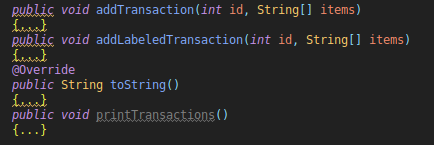
\includegraphics[width=0.75\linewidth]{apriori/images/data_structs/instance/methods.png}
			\end{figure}
			\par, les deux premières méthodes \textbf{addTransaction} et \textbf{addLabeledTransaction} font respectivement office d'interface pour ajouter une transaction à l'un des deux attributs (pour assurer une transparence d'utilisation de la classe). Les deux autres méthodes sont des méthodes d'affichage pour un éventuel débogage de l'application.
			
			\subsection{AprioriInstanceReader :} \label{loader} c'est la classe qui va construire une objet de la classe \textbf{InstanceApriori} à partir d'un fichier d'extension \textbf{.arff}, ou bien à partir d'un objet de la classe \textbf{weka.Instances} classe déjà existant.
			\par Les attributs sont les suivants : 
			\begin{figure}[H]
				\centering
				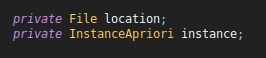
\includegraphics[width=0.75\linewidth]{apriori/images/data_structs/laoder/properties.png}
			\end{figure}
			\par l'attribut \textbf{instances} est donc un objet de la classe \textbf{InstanceApriori} vu précédemment, l'autre est un objet qui stock le descripteur du fichier \textbf{.arff}.
			
			\par 
			Les méthodes sont celles mentionnées dans \ref{loader}, voici leurs prototypes :
			\begin{figure}[H]
				\centering
				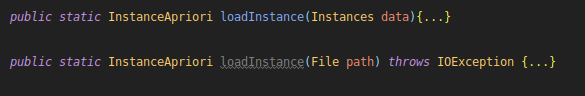
\includegraphics[width=0.75\linewidth]{apriori/images/data_structs/laoder/methods.png}
			\end{figure}
			
			\subsection{Searcher :} 
			Cette classe est celle qui va contenir à la fois les données en entré (Instance et ses méta-donnés), les hyper paramètres ainsi que le résultat de l'algorithme (Itemsets fréquents et règles d'association).
			\par
			Les attributs sont les suivants 
			\begin{figure}[H]
				\centering
				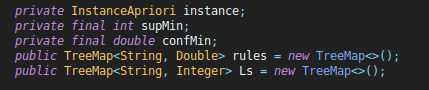
\includegraphics[width=0.75\linewidth]{apriori/images/data_structs/searcher/props.png}
			\end{figure}
			\par Les trois premiers sont triviaux (voir \ref{loader}), les deux derniers sont respectivement : une structure de hachage de la règle d'association à son degré de confiance \textbf{Règle -> Confiance} pour l'attribut \textbf{rules}, et une structure de hachage d'un itemset à sa fréquence d'apparition \textbf{Itemset -> Support}, et cela pour garantir un accès directe l'information désirée.
			
			\par 
			Pour ce qui est des méthodes, il en existe trois catégories :
			\begin{itemize}
				\item \textbf{Méthode principale} : essentiel au fonctionnement de l'algorithme. La seule méthode répondant à cette description est la méthode \textbf{search} : 
				\begin{figure}[H]
					\centering
					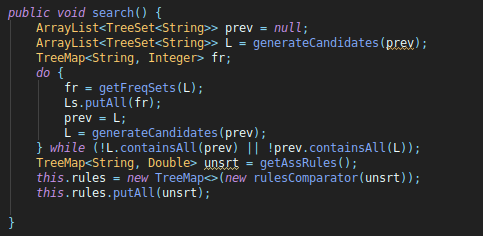
\includegraphics[width=0.6\linewidth]{apriori/images/data_structs/searcher/search.png}
				\end{figure}
				\item \textbf{Méthode d'aide} : pour modulariser le traitement d'une méthode principale, les méthodes suivantes ont font partie : 
				\begin{figure}[H]
					\centering
					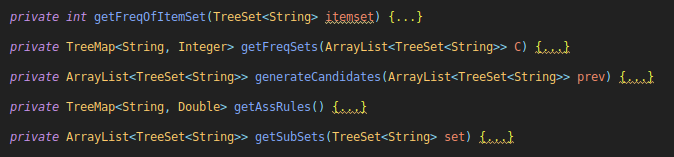
\includegraphics[width=0.75\linewidth]{apriori/images/data_structs/searcher/helpers.png}
				\end{figure}
				\par Dans l'ordre le rôle de chacune est le suivant :
				\begin{itemize}
					\item \textbf{getFreqOfItemSet} Calcule le support d'un itemset
					\item \textbf{getFreqSets} Extrait les itemset fréquents ( dont le support dépasse le support minimum)
					\item \textbf{generateCandidates} Génère un nouveau itemset candidat en combinant les item d'un itemset antérieur.
					\item \textbf{getAssRules} Extrait les règles d'association à partir des itemset fréquents extraits au préalable.
					\item \textbf{getSubSets} Extrait l'ensemble des parties d'ensemble d'un itemset. 
				\end{itemize}
				\item \textbf{Méthode deboggage} : principalement servant à afficher de manière structurée les résultats finaux ou intermédiaire d'un des types de méthodes cités. Nous y trouvons les méthodes : 
				\begin{figure}[H]
					\centering
					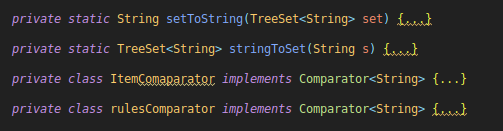
\includegraphics[width=0.75\linewidth]{apriori/images/data_structs/searcher/printers.png}
				\end{figure}
			\end{itemize}
		
	\section{Interface graphique}
		\paragraph{}
		Nous avons intégré l'interface graphique pour l'utilisation d'algorithme \textbf{Apriori} dans l'interface principale, pour que l'utilisateur puisse lancer le traitement sur une datase préalablement traité (nettoyage et remplissage de valeur manquantes), voici l'interface choisie suivit de quelques explications : 
		\begin{figure}[H]
			\centering
			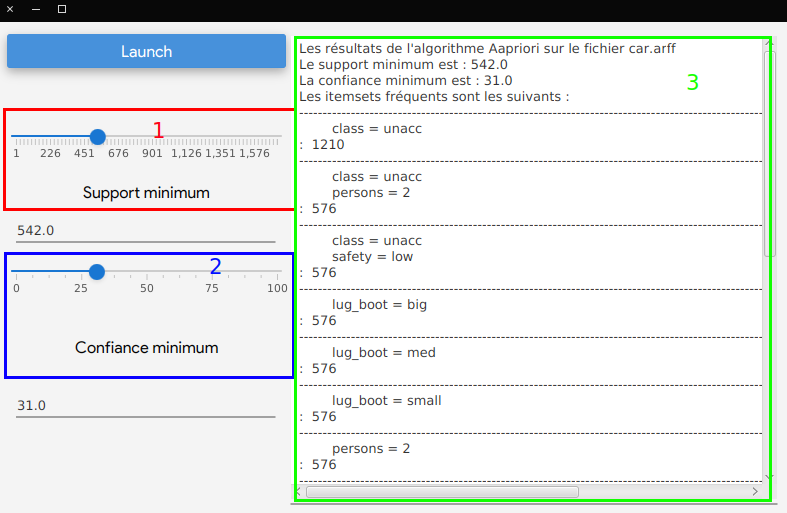
\includegraphics[width=0.75\linewidth]{apriori/images/apriori.png}
		\end{figure}
		\paragraph{}
		L'interface se compose de 3 zones :
		\begin{itemize}
			\item \textbf{Zone 1 et 2:} permettre d'introduire les valeurs des hyper paramètres
			\item \textbf{Zone 3:} affichage du résultat comme une liste d'itemsets fréquents suivie d'une liste de règle d'association. 
		\end{itemize}
		
	\section{Résultats expérimentaux}
		\subsubsection{Choix du dataset}
			\paragraph{}
			Pour tester le comportement de notre implémentation de l'algorithme apriori, nous avons choisi de le tester sur un dataset purement nominal (\textbf{car.arff}).
		\subsubsection{Variations des paramètres}
			\paragraph{}
			Nous avons choisi de faire varier les deux paramètres qui sont supMin et confMin de façon automatique, la plage du premier est l'intervalle $\left[ \text{0.1*\textbf{nombreInstance} , \textbf{nombreInstance}} \right]$ avec un pas $step = \frac{ nombreInstance}{10}$.
			\par 
			La plage du 2e est l'intervalle suivant : $\left[ 0.5 , 1\right]$ avec un pas $step = 0.1$
		\subsubsection{Résultats}
			\paragraph{}
			Les résultats sont récapitulé dans le tableau suivant : 
			% Please add the following required packages to your document preamble:
			% \usepackage[table,xcdraw]{xcolor}
			% If you use beamer only pass "xcolor=table" option, i.e. \documentclass[xcolor=table]{beamer}
			\begin{table}[H]
				\centering
				\begin{tabular}{|c|c|c|c|c|}
					\hline
					\textbf{supMin} & \textbf{confMin} & \textbf{nombre itemset freq} & \textbf{nombre de règle d'ass} & \textbf{temps (ms)} \\ \hline
					172             & 0.5              & 86                           & 22                             & 410            \\ \hline
					172             & 0.6              & 86                           & 14                             & 431            \\ \hline
					172             & 0.7              & 86                           & 6                              & 433            \\ \hline
					172             & 0.8              & 86                           & 2                              & 388            \\ \hline
					172             & 0.9              & 86                           & 1                              & 382            \\ \hline
					344             & 0.5              & 31                           & 6                              & 41             \\ \hline
					344             & 0.6              & 31                           & 6                              & 42             \\ \hline
					344             & 0.7              & 31                           & 3                              & 44             \\ \hline
					344             & 0.8              & 31                           & 2                              & 40             \\ \hline
					344             & 0.9              & 31                           & 1                              & 47             \\ \hline
					516             & 0.5              & 12                           & 1                              & 36             \\ \hline
					516             & 0.6              & 12                           & 1                              & 39             \\ \hline
					516             & 0.7              & 12                           & 1                              & 38             \\ \hline
					516             & 0.8              & 12                           & 1                              & 37             \\ \hline
					516             & 0.9              & 12                           & 1                              & 39             \\ \hline
					688             & 0.5              & 1                            & 0                              & 43             \\ \hline
					\rowcolor[HTML]{9AFF99} 
					...             & ...              & ...                          & ...                            & ....           \\ \hline
					1204            & 0.9              & 1                            & 0                              & 35             \\ \hline
					\rowcolor[HTML]{9AFF99} 
					...             & ...              & ...                          & ...                            & ...            \\ \hline
					1720            & 0.9              & 0                            & 0                              & 33             \\ \hline
				\end{tabular}
				\caption{Tableau récapitulatif des résultats de l'algorithme apriori sur le dataset \textbf{car.arff}}
				\label{my-label}
			\end{table}
			\paragraph{Remarques :} Les valeurs en vert désignent un stagnation des valeurs \textbf{nombre itemset freq} et \textbf{nombre de règle d'ass}
		\subsection{Commentaires}
			\paragraph{}
			D'après le tableau, il est notable que le paramètre qui influe le plus sur le temps d'exécutions est le \textbf{support minimum}, c'est facilement remarquable si on prend une valeur fixe pour ce dernier en faisant varier l'autre paramètre \textbf{Confiance minimum}, par exemple : \\
			\[
				\text{Si } supMin = 344 \text{ et } \forall confMin \rightarrow temps \in \left[ 40,47\right]
			\]
			Cela montre que la plus part des ressources sont mobilisé pour l'extraction des itemsets fréquents.
			\par Il est aussi a noté que plus le support minimum augmente ( on impose donc un forte condition sur la fréquence d'apparitions des itemsets) le nombre d'itemsets fréquent ainsi que le nombre de règles d'association ainsi que le temps de calcul diminuent en conséquence.

	
\newpage
\chapter{Classification à l'aide de l'algorithme K plus proches voisins (KNN)}
	\section{Introduction}
	\section{Définitions}
		\paragraph{}
		\subsection{Point}
			\paragraph{}
		\subsection{Distance}\label{transaction}
			\paragraph{}
		\subsection{Voisinage}
			\paragraph{}
		\subsection{Classification}
	
	\section{Algorithme}
		\paragraph{}
	\section{Implémentation}
		\subsection{Langage de programmation}
		\subsubsection{Schémas d'exécution}
		\subsubsection{Structures de données}
	\section{Interface graphique}
	
	\section{Résultats expérimentaux}
		\subsubsection{Choix du dataset}
		\subsubsection{Variations des paramètres}
		\subsubsection{Résultats}
	\subsubsection{Commentaires}
	
	\section{Conclusion}

\newpage
\chapter{Clustering à l'aide de l'algorithme DBSCAN}\label{dbscan}
\section{Introduction}
	Quand nous somme face à un gros ensemble de données dont nous connaissons les caractéristiques mais pas les relations qui lient chaque individu d'un échantillon, nous voudrions être capable de regrouper les instances (point,individu ...) qui sont similaires (petites distances entre eux) dans un sous ensemble bien défini, ce processus est plus communément appelé \textbf{Clustering}.
	\par De manière informelle, le clustering est l'opération de regroupement d'objets dans un groupe compacte nommé \textbf{Cluster} de telle sorte que les membres d'un même cluster soient similaire à un certain point, et arbitrairement différents (grandes distances) des objets d'un autre cluster.
	\par 
	Il existe une multitude d'algorithme de clustering, nous avons décidé d'implémenter l'algorithme Density-based spatial clustering of applications with noise (DBSCAN) pour analyser son comportement, et ainsi critiquer ses forces, ses faiblesses et ainsi pouvoir l'utiliser dans des domaines qui lui conviendraient.
\section{Définitions}
	\paragraph{}
	Comme pour les chapitres précédents, nous allons donner quelques définitions pour faciliter la compréhension de l'algorithme, il est a noté que nous utiliserons quelques définitions du chapitre précédent, notamment (\ref{point} \ref{distance} \ref{neighborhood})
	\subsection{E-voisinage}
		\paragraph{}
		Semblable à la notion de voisinage vu dans \ref{neighborhood}, le e-voisinage d'un point $P$ appartenant un ensemble de points $E$ est l'ensemble $V_\epsilon$ des points qui sont à une distance $D \leq \epsilon$, plus formellement : 
		\[
			V_\epsilon(P) = \lbrace x \in E | D_2(P,x) \leq \epsilon \rbrace
		\] 
		\par De plus si $P$ est un \textbf{core-point} (voir \ref{corepoint}) alors l'ensemble $V_\epsilon$ formera un ensemble de points \textbf{directement-atteignables}.
	\subsection{Core-point}\label{corepoint}
		\paragraph{}
		Un core-point, selon l'algorithme \textbf{DBSCAN} est un point $P_c$ dans l'ensemble $E$ dont le cardinal de son E-voisinage est supérieure ou égale à une constante $minPts = k$, l'ensemble de ces core-points formera un ensemble que l'on dénotera $E_c$, plus formellement
			\[
				E_c = \lbrace P \in E | k \leq |V_\epsilon(P)| \rbrace
			\]
		Les éléments du e-voisinage d'un core-point $P$ sont des points qui sont directement-atteignables par ce point.
	\subsection{Point de bord (Border-point)}
		\paragraph{}
		Un point de bord est un point $P_b$ dans l'ensemble $E$ dont le cardinal de son E-voisinage est inférieure au paramètre $k$ et il existe un core-point $P_c$ qui est dans ce même E-voisinage. L'ensemble de ces border-points formera un ensemble que l'on dénotera $E_cb$, plus formellement : 
		\[
			E_b = \lbrace P \in E | k \geq |V_\epsilon(P)| \land \exists P_c \in V_\epsilon(P) \bigcap E_c \rbrace
		\] 
	\subsection{Bruit}
		\paragraph{}
		Un point $P$ est considéré comme étant du bruit $P_n$s'il n'est ni un core-point ni un border-point, il appartiendra à un ensemble $E_n$ tel que : 
		\[
			E_n = \lbrace P \in E | P \notin E_c \land P \notin E_b \rbrace
		\] 
	\subsection{Cluster}
		\paragraph{}
		Un cluster $C$ est un ensemble de points dont  un algorithme de clustering a déterminé qu'ils étaient similaires dans un certain sens, on peut donc dire que c'est l'ensemble des points dont la similarité est très forte, et dont la similarité avec les points d'autres clusters $C\prime \neq C$ est très faible.	
	\subsection{Centre de gravité}
		\paragraph{}
		Le centre d'un gravité d'un cluster $C$ est un point $G_C$ (qui n'existe pas forcement dans le cluster) qui sera désigné comme représentant de ce dit cluster, il existe beaucoup de façons de le déterminer, une des façon de le faire est l'utilisation de la formule suivante : 
		
		\[
			G_C = (\frac{\sum_{i=1}^{N} x_{i,1}}{N} , ... , \frac{\sum_{i=1}^{N} x_{i,M}}{N})
		\]
		Avec : 
		\begin{itemize}
			\item $N$ : le nombre de points dans le cluster.
			\item $M$ : le nombre d'attributs d'un point dans le cluster.
		\end{itemize}
		
		\paragraph{}
		De même nous pouvons définir le centre de gravité du nuage de points en entier, en considérant $G$ l'ensemble des centres de gravité de chaque clusters $C$, soit $G_{pts}$ le point que nous cherchons, ce sera le centre de gravité de l'ensemble $G$, donc :
		\[
				G_{pts} = (\frac{\sum_{i=1}^{N_G} x_{i,1}}{N_G} , ... , \frac{\sum_{i=1}^{N_G} x_{i,M}}{N_G})
		\]
		où 
		\begin{itemize}
			\item $N_G$ : le nombre de points dans $G$.
			\item $M$ : le nombre d'attributs d'un centre de gravité.
		\end{itemize}
		\par 
		Voici un schema pour illustrer cela :
		\begin{figure}[H]
			\centering
			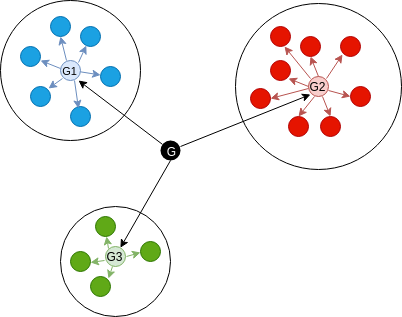
\includegraphics[width=0.60\linewidth]{dbscan/images/clusters.png}
			
		\end{figure}
	\newpage
	\subsection{Inerties}
		 Pour quantifier la similarité (inversement la dissimilarité) au sein d'un cluster, et a travers les clusters, nous avons décidé d'utiliser les deux mesures suivantes : 
		 
		 \subsubsection{Inertie intra-classes}
		 	\paragraph{}\label{inertie}
		 	C'est une quantité qui détermine a quel point les éléments d'un cluster sont proches les uns des autres, elle est calculé en sommant les carrés des distances entre ces points et le centre de gravité d'un cluster. Nous disposons d'un ensemble de clusters $C$, dont les centres de gravité seront notés $G_{C_i}$, on définira l'inertie d'un cluster $C$ comme étant : 
		 	\[
		 		Iner(C_i) = \sum_{x \in C_i } D_2(x,G_{C_i})^2
		 	\]
		 	Par la suite, l'inertie intra-classe d'un ensemble de clusters $C$  comme étant la somme des inerties des clusters le composant : 
		 	\[
		 		Intra(C) = \sum_{C_i \in C} iner(C_i) 
		 	\]
		 	\par De ce fait, plus cette quantité est petite, plus les éléments de chaque cluster sont proches les un des autres, c'est donc une quantité a minimiser par un algorithme de clustering.
		 	
		 \subsubsection{Inertie inter-classes}
			 \paragraph{}
			 C'est une quantité qui détermine a quel point les éléments d'un cluster sont loins des éléments des autre clusters,elle est calculé en sommant les carrés des distances entre les centre de gravités de chaque cluster avec le centre de gravité du nuage de points $G_{pts}$, Nous disposons d'un ensemble de clusters $C$, dont les centres de gravité seront notés $g \in G_c$ , on définira l'inertie inter-classe d'un ensemble de cluster $C$ comme étant : 
			 \[
			 Inter(C) = \sum_{g \in G_C } D_2(g,G_{pts})^2
			 \]
			 \par De ce fait, plus cette quantité est grande, plus les éléments de chaque cluster sont loins par rapport aux éléments des autre clusters, , c'est donc une quantité a maximiser par un algorithme de clustering.
\section{Algorithme}
	\paragraph{}
		Le principe de l'algorithme est assez simple, en commençant d'un core-point arbitraire, il essayera de construire un cluster incluent ce point et tout les points indirectement-atteignables à partir de lui même, en marquant chaque point visité pour ne pas le retraiter par la suite, les limites d'un cluster seront donc délimités par les border-points, ainsi, les clusters seront formés de points très proches les uns des autres (d'après la définition des points directement(indirectement)-atteignables), ce qui aura pour effet de construire des clusters très \textbf{Denses}. Le pseudo code est le suivant : 
		\par 
		Algorithme principal : \\
		\begin{algorithm}[H]
			\caption{DBSCAN}
			\SetKwInOut{Input}{Entrée}\SetKwInOut{Output}{Sortie}
			\SetKwFunction{neigh}{E-Voisinage}
			\SetKwFunction{exp}{EtendreCluster}
			
			\Input{(E : Ensemble des instances, $\epsilon$ : réel, minPts : entier)}
			\Output{(C : Ensemble des clusters)}
			$C \gets 0 $ ;\\
			$NV \gets E$ Ensemble des points non visités ;\\
			$V \gets \emptyset$ Ensemble des points visités ;\\
			$N \gets \emptyset $ Ensemble des points bruits ;\\
			\ForEach{$p \in NV$}
			{
				$NV \gets NV -\lbrace p \rbrace$ ;\\
				$V \gets V  \bigcup \lbrace p \rbrace$ ;\\
				$Voisinage \gets $ \neigh{$p,\epsilon$} ;\\
				\eIf{$|Voisinage| < minPts$}
				{
					$N \gets N \bigcup \lbrace p \rbrace$ ;\\
				}
				{
					$C \gets C + 1 $;\\
					\exp{$p , Voisinage , C , \epsilon , minPts$}
				}
				
			}
			\KwRet{$C$}		
		\end{algorithm}
		
		\begin{procedure}[H]
			\SetKwFunction{neigh}{E-Voisinage}
			
			$C \gets C \bigcup \lbrace p \rbrace$ \;
			\ForEach{$v \in Voisinage$}
			{
				\If{$v \notin V$}
				{
					$NV \gets NV -\lbrace v \rbrace$ \;
					$V \gets V  \bigcup \lbrace v \rbrace$ \;
					$Vosinage \prime \gets $ \neigh{$v,\epsilon$}\;
					\If{$|Voisinage \prime | \geq minPts$}
					{
						$Voisinage \gets Voisinage \bigcup Voisinage \prime $\;
					}
				}
				\If{$v \notin C \forall C \in Clusters$}
				{
					$C \gets C \bigcup \lbrace v \rbrace$ \;
				}
			}
			\caption{EtendreCluster((p : Point, Voisinage : ensemble, C : cluster, $\epsilon$ : réel, minPts : entier))}
		\end{procedure}
		
		
		
	\section{Implémentation}
		\paragraph{}
		Pour mieux visualiser la structure interne de notre implémentation, nous allons présenter d'abord un diagramme \textbf{UML} puis ensuite détailler les composants du module \textbf{DBSCAN} : 
		\begin{figure}[H]
			\centering
			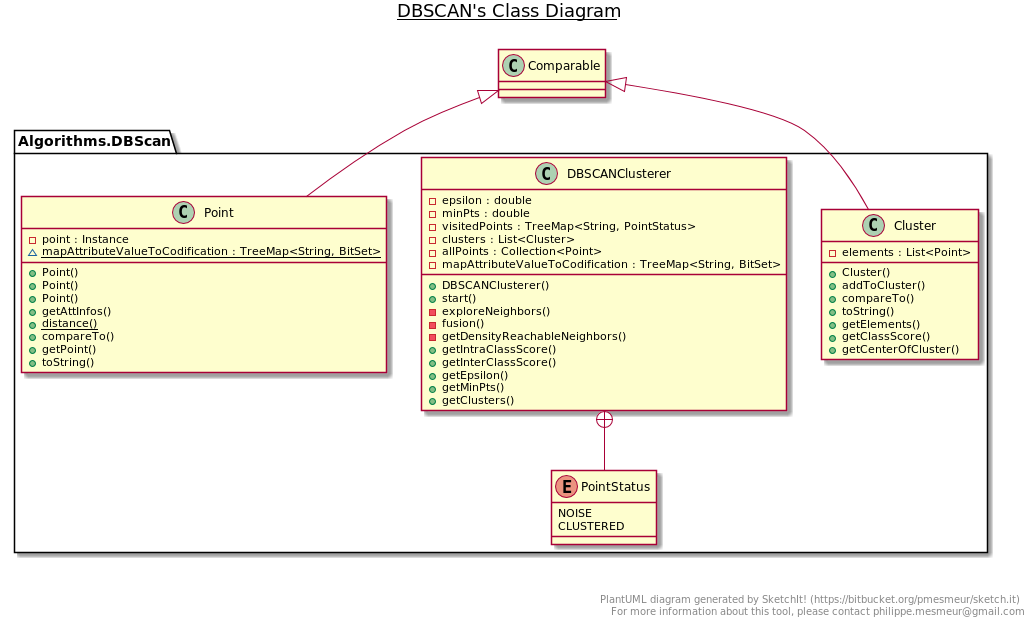
\includegraphics[width=\linewidth]{dbscan/images/uml.png}
		\end{figure}
		\par 
		Le module se compose donc de trois grande classes : 
		\begin{itemize}
			\item \textbf{Point} qui servira d'encapsulation à la notion de point dans un dataset, utilisant des méthodes de manipulation d'un point ou de points.
			\item \textbf{Cluster} qui servira d'encapsulation à la notion de cluster comme étant un ensemble d'objets de la classe \textbf{Point}, utilisant des méthodes de manipulation de clusters et de calcul des centre de gravité.
			\item \textbf{DBSCANClusterer} qui est la classe qui va effectuer le travail de clustering en manipulant les objets des deux classes précédentes.
		\end{itemize}
	
	\subsection*{Point}
		\paragraph{}
		\begin{itemize}
			\item Nous commençons par détailler les attributs de la classe : 
			\begin{figure}[H]
				\centering
				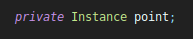
\includegraphics[width=0.75\linewidth]{dbscan/images/point/props.png}
			\end{figure}
			\par L'unique attribut de la classe st un objet de la classe \textbf{weka.instance}, car à la base un point est une instance du dataset.
			
			\item Les méthodes implémentées sont les suivantes : 
			\begin{figure}[H]
				\centering
				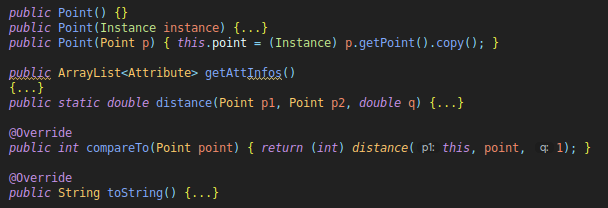
\includegraphics[width=0.75\linewidth]{dbscan/images/point/meths.png}
				
			\end{figure}
			\begin{itemize}
				\item \textbf{Point()} Ce sont les différents constructeur de la classe qui instancient soit avec une valeur nulle, à partir d'un objet de la classe \textbf{weka.Instance} ou bien en copiant les attribut d'un objet de la classe \textbf{Point}
				\item \textbf{getAttInfos} Une méthode d'aide qui retourne la liste des attributs d'une instance.
				\item \textbf{Distance} la méthode de calcul de la p-distance \ref{distance} entre deux points ( instances ) données
				\item \textbf{compareTo} implémentation de la méthode compareTo de l'interface \textbf{Comparable} pour qu'on puisse comparer deux objets de la classe Point.
			\end{itemize}
			
		\end{itemize}
	\subsection*{Cluster}
		\paragraph{}
		\begin{figure}[H]
			\centering
			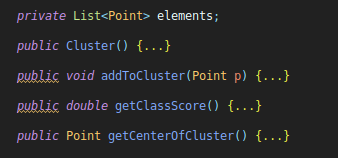
\includegraphics[width=0.75\linewidth]{dbscan/images/cluster/all.png}
		\end{figure}
		\begin{itemize}
			\item L'unique attribut de la classe st une liste d'objets de la classe \textbf{Point}, car un cluster est un ensemble de points.
			
			\item Les méthodes implémentées sont les suivantes : 
			\begin{itemize}
				\item \textbf{Cluster()} Le constructeur de la classe qui initialise la liste de points.
				\item \textbf{addToCluster} Méthode d'aide qui ajoute un point au cluster.
				\item \textbf{getCenterOfCluster} la méthode qui calcul le centre de gravité du cluster.
				\item \textbf{getClassScore} méthode qui retourne la valeur de l'inertie intra-classe du cluster.
			\end{itemize}
		\end{itemize}
	
	\subsection*{DBSCANClusterer}
		\begin{itemize}
			\item Nous commençons par détailler les attributs de la classe : 
			\begin{figure}[H]
				\centering
				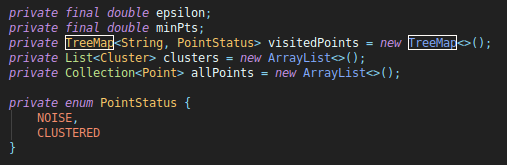
\includegraphics[width=0.75\linewidth]{dbscan/images/dbscan/props.png}
			\end{figure}
			\begin{itemize}
				\item \textbf{epsilon} et \textbf{minPts} sont les deux paramètre de l'algorithme.
				\item \textbf{visitedPoint} une structure de hachage qui associe à chaque point son status (Dans un cluster ou Bruit).
				\item \textbf{clusters} une liste d'objets de la classe Cluster qui contiendra les clusters construits par l'algorithme.
				\item \textbf{allPoints} l'ensemble des points du dataset.
			\end{itemize}
			\item Les méthodes implémentées sont les suivantes : 
			\begin{itemize}
				\item \begin{figure}[H]
					\centering
					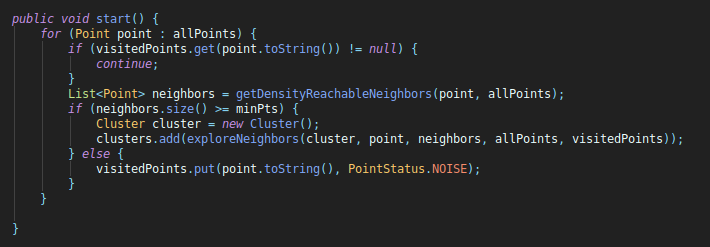
\includegraphics[width=0.75\linewidth]{dbscan/images/dbscan/start.png}
				\end{figure} \textbf{start : } c'est la boucle principale de l'algorithme qui va parcourir l'ensemble des points pour former les clusters.
			
				\item \begin{figure}[H]
					\centering
					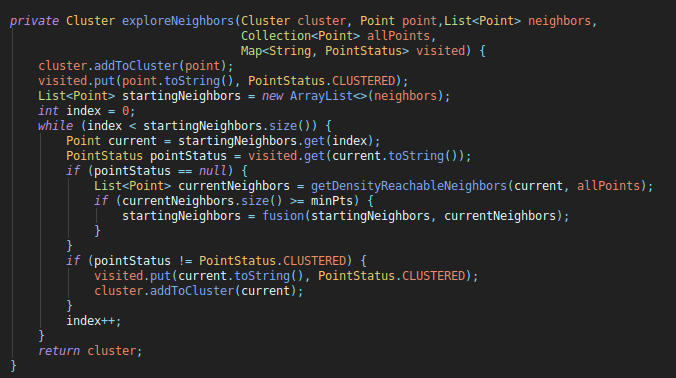
\includegraphics[width=0.75\linewidth]{dbscan/images/dbscan/expand.png}
				\end{figure} \textbf{exploreNeighbors : } c'est la procédure \textbf{étendreCluster} vu précédemment, elle va chercher à rassembler tout les points indirectement-atteignables depuis un point donné pour former un nouveau cluster.
			
				\item \begin{figure}[H]
					\centering
					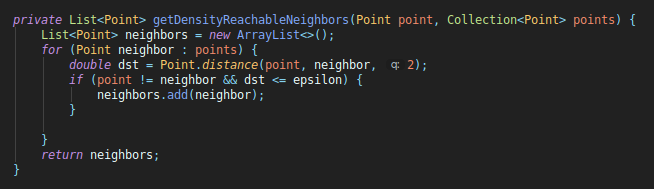
\includegraphics[width=0.75\linewidth]{dbscan/images/dbscan/neighborhood.png}
				\end{figure} \textbf{getDensityReachableNeighbors : } c'est la procédure \textbf{E-voisinage} vu précédemment, elle va retourner l'ensemble des points directement-atteignable depuis le point donné.
				
				\item \begin{figure}[H]
					\centering
					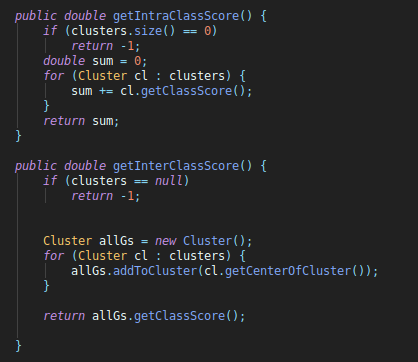
\includegraphics[width=0.55\linewidth]{dbscan/images/dbscan/score.png}
				\end{figure} 
				\begin{itemize}
					\item \textbf{getIntraClassScore} elle va calculer l'inertie intra-classes des clusters.
					\item \textbf{getInterClassScore} elle va calculer l'inertie du cluster formé des centres de gravité de chaque cluster, donc l'inertie inter-classes.
				\end{itemize}
			\end{itemize}
			
		\end{itemize}
\section{Interface graphique}
	\paragraph{}
	De manière analogue à ce que nous avons fait pour les modules précédents (\ref{apriori} \ref{knn}) Nous avons intégré à l'interface graphique principale l'algorithme \textbf{DBSCAN}, voici l'interface choisie suivie de quelques explications : 
	\begin{figure}[H]
		\centering
		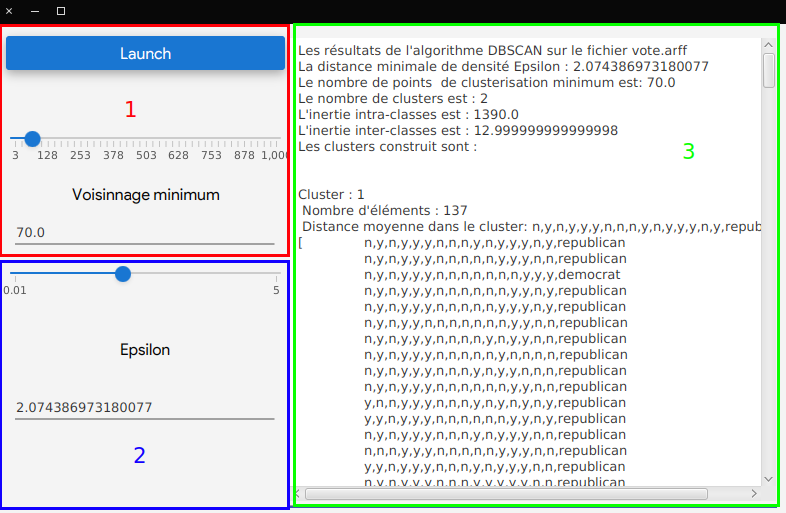
\includegraphics[width=0.75\linewidth]{dbscan/images/app.png}
	\end{figure}
	\paragraph{}
	L'interface se compose de 3 zones :
	\begin{itemize}
		\item \textbf{Zone 1 et 2:} permettre d'introduire les valeurs des hyper paramètres $\epsilon$ et minPts.
		\item \textbf{Zone 3:} affichage du résultat comme une liste de clusters avec les points qui les composent, ainsi que les valeurs des inerties inter et intra-classes.
	\end{itemize}
\section{Résultats expérimentaux}
	\subsection{Choix du dataset}
		\paragraph{}Nous avons choisi de tester le comportement de l'algorithme dans les deux cas oû les données sont soit purement numériques soit purement nominales : 
		\begin{itemize}
			\item Dataset purement numérique : nous avons choisis le dataset \textbf{iris.arff}
			\item Dataset purement nominal : nous avons choisis le dataset \textbf{vote.arff}
		\end{itemize}
	\subsection{Variations des paramètres}
		\paragraph{}
			Pour ce qui est des paramètres, nous avons décidé de faire varier le nombre de points minimum \textbf{minPts} car il affecte grandement le choix d'un point comme core-point, il prendra ses valeurs dans l'intervalle $\left[ 0.1*\text{nbrInstance} , \frac{\text{nbrInstance}}{3}\right]$ avec un pas $step = \frac{\text{nbrInstance}}{10}$.
			\par 
			Le 2e paramètre $\epsilon$ quantifiera la notion de \textbf{densité} dans le nuage de point, en effet si la valeur de paramètre est grande, l'algorithme tendra à considérer des points assez distants de lui comme étant \textbf{proches}. Malheureusement la normalisation de valeurs d'attributs des points ne garanti pas qu'on aura une distance qui sera elle aussi normalisée, pour illustrer cela nous allons prendre l'exemple suivant : 
			\par
			Posons : 
			\[
				X = (x_1,...,x_n)
			\]
			et
			\[
				Y = (y_1,...,y_n)
			\]
			Deux points de l'ensemble des points $E$.\\
			Si on pose $x_i,y_i \in [0,1],\forall i =1..n$, Plus particulièrement donnons à chaque attribut $x_i$ la valeur $0.5$, et à chaque attribut $y_i$ la valeur $1$ ainsi
			$x_i = 1, y_i = 0.5, \forall i =1..n$, et posons $n=10$ le nombre d'attributs, ainsi la formule de la 2-distance \ref{distance} deviendra : 
			
			\begin{flalign}\label{proof}
			D_2(X,Y) &= \sqrt{\sum_{i=1}^{10} (1-0.5)^2} \\
			D_2(X,Y) &= \sqrt{\sum_{i=1}^{10} 0.25} \\
			D_2(X,Y) &= \sqrt{10*0.25}\\
			D_2(X,Y) &= \sqrt{2.5}\\
			D_2(X,Y) &\approx 1.58 \notin [0,1]
			\end{flalign}
			Ainsi nous pouvons aussi déduire que l'inertie intra-classe peut facilement exploser en terme de grandeur, une preuve sera présentée dans (REEEEEEEEEEEEEEEEEEEEEEEEEEEEEEEEFFFF). Pour ce qu'il en est de la variation de ce paramètre, nous partons du postulat que si nous disposons d'un ensemble de points avec $n$ attributs \textbf{normalisés}, deux des points les plus éloignés peuvent êtres (dans le cas numérique) :
			$X=(0,...,0)$ et $Y=(1,...,1)$ (tout les attributs a distance maximale) , la distances les séparant sera donc $D_2(X,Y) = \sqrt{n}$, donc le paramètre $\epsilon$ sera dans l'intervalle $\left[ \frac{\sqrt{n}}{10} , \sqrt{n}\right]$, avec un pas $step = \frac{\sqrt{n}}{20}$.
	\subsection{Résultats}
		\paragraph{}
		Nous avons lancé l'algorithme sur les datasets mentionnés plus haut en gardant à chaque fois les informations nécessaires pour comparer les résultats (nombre de clusters,inerties inter-intra classes, temps ...), les tableaux comparatifs suivants résument le processus, ils serons ensuite accompagnés de quelques commentaires :
		\paragraph{Remarques} 
		Dans le cas où aucun cluster n'est construit les deux mesures de performances vaudront -1.
		\subsubsection*{Résultats pour iris.arff }
		
		\begin{table}[H]
			\centering
			\begin{tabular}{|c|c|c|c|c|c|}
				\hline
				\textbf{$\epsilon$} & \textbf{minPts} & \textbf{Nb cluster} & \textbf{L'inertie intra-classes} & \textbf{L'inertie inter-classes} & \textbf{temps} \\ \hline
				0,111803399         & 5               & 5                   & 2,062029911                      & 4,361321025                      & 8              \\
				0,111803399         & 10              & 1                   & 0,907413281                      & 0                                & 4              \\
				0,111803399         & 15              & 1                   & 0,315181554                      & 0                                & 5              \\
				0,223606798         & 5               & 2                   & 18,62857928                      & 0,85701552                       & 5              \\
				0,223606798         & 10              & 2                   & 18,00560921                      & 0,85701552                       & 6              \\
				0,223606798         & 15              & 2                   & 13,04401911                      & 0,715499107                      & 5              \\
				0,223606798         & 20              & 2                   & 10,41219874                      & 0,715499107                      & 5              \\
				0,223606798         & 25              & 2                   & 7,711637591                      & 0,823875133                      & 6              \\
				0,223606798         & 30              & 2                   & 3,223514733                      & 0,611410909                      & 4              \\
				0,223606798         & 35              & 2                   & 2,408509621                      & 0,702501631                      & 5              \\
				0,223606798         & 40              & 0                   & -1                               & -1                               & 5              \\
				0,223606798         & 45              & 0                   & -1                               & -1                               & 3              \\
				0,335410197         & 5               & 2                   & 19,50523183                      & 0,85701552                       & 6              \\
				...                 & ...             & ...                 & ...                              & ...                              & ...            \\
				0,335410197         & 30              & 2                   & 19,17890257                      & 0,85701552                       & 4              \\
				0,335410197         & 35              & 2                   & 14,3095591                       & 0,715499107                      & 6              \\
				0,335410197         & 40              & 2                   & 13,49945477                      & 0,715499107                      & 6              \\
				0,335410197         & 45              & 2                   & 13,2196536                       & 0,715499107                      & 6              \\
				0,447213595         & 5               & 2                   & 19,50523183                      & 0,85701552                       & 5              \\
				...                 & ...             & ...                 & ...                              & ...                              & ...            \\
				0,447213595         & 45              & 2                   & 19,50523183                      & 0,85701552                       & 6              \\
				0,559016994         & 5               & 1                   & 101,5489152                      & 0                                & 5              \\
				...                 & ...             & ...                 & ...                              & ...                              & ...            \\
				2,124264579         & 45              & 1                   & 101,5489152                      & 0                                & 5              \\ \hline
			\end{tabular}
			\caption{Résultats de l'algorithme DBSCAN sur le dataset iris.arff}
		\end{table}
		\paragraph{Commentaires}
			Nous pouvons extraire de ce tableau que le meilleur couple de paramètre est celui tout en haut du tableau, car il construit plusieurs cluster, et minimise l'inertie intra-classe tout en maximisant l'inertie interclasse. Il est a noter que dans certains cas, on peut tomber sur une valeur très grande pour l'inertie intra-classe, en effet comme nous l'avons démontré dans \ref{proof}, une distance de deux points normalisés peut dépasser 1, si on considère la formule de l'inertie d'une classe vu dans  \ref{inertie}, qui est la somme d'un nombre de carrés de distances égal au nombre de points dans un cluster, nous pouvons facilement atteindre des valeurs très grandes, les principales causes sont donc un très grand nombre d'attributs et un très grande nombre de points dans un même cluster. Ceci peu expliquer une très grande différence entre les deux mesures de performance, mais ceci importe peu car le but n'est pas de minimiser la différence absolue entres ces deux valeurs, mais de considérer chaque valeur comme un objectif à minimiser ou à maximiser, c'est donc une fonction à double objectifs que nous voulons optimiser.
		\subsubsection*{Résultats pour vote.arff }
		
		% Please add the following required packages to your document preamble:
		% \usepackage[table,xcdraw]{xcolor}
		% If you use beamer only pass "xcolor=table" option, i.e. \documentclass[xcolor=table]{beamer}
		\begin{table}[H]
			\centering
			\begin{tabular}{|c|c|c|c|c|c|}
				\hline
				\textbf{$\epsilon$} & \textbf{minPts} & \textbf{Nb cluster} & \textbf{\begin{tabular}[c]{@{}c@{}}L'inertie \\ intra-classes\end{tabular}} & \textbf{\begin{tabular}[c]{@{}c@{}}L'inertie \\ inter-classes\end{tabular}} & \textbf{temps} \\
				1,236931688         & 14              & 2                   & 273                                                                         & 14                                                                          & 606            \\
				1,236931688         & 28              & 2                   & 86                                                                          & 14                                                                          & 620            \\
				\rowcolor[HTML]{9AFF99} 
				1,236931688         & 42              & 2                   & 16                                                                          & 14                                                                          & 612            \\
				1,64924225          & 14              & 2                   & 902                                                                         & 13                                                                          & 619            \\
				1,64924225          & 28              & 2                   & 709                                                                         & 13                                                                          & 615            \\
				1,64924225          & 42              & 2                   & 640                                                                         & 13                                                                          & 617            \\
				1,64924225          & 56              & 2                   & 375                                                                         & 13                                                                          & 621            \\
				1,64924225          & 70              & 2                   & 314                                                                         & 13                                                                          & 617            \\
				2,061552813         & 56              & 2                   & 1399                                                                        & 13                                                                          & 628            \\
				2,061552813         & 70              & 2                   & 1390                                                                        & 13                                                                          & 621            \\
				2,061552813         & 84              & 2                   & 1341                                                                        & 13                                                                          & 620            \\
				2,061552813         & 98              & 2                   & 1285                                                                        & 13                                                                          & 621            \\
				2,061552813         & 112             & 2                   & 1193                                                                        & 13                                                                          & 621            \\
				2,061552813         & 126             & 2                   & 1042                                                                        & 14                                                                          & 615            \\
				2,061552813         & 140             & 2                   & 977                                                                         & 14                                                                          & 611            \\
				1,64924225          & 84              & 1                   & 134                                                                         & 0                                                                           & 615            \\
				2,061552813         & 14              & 1                   & 2395                                                                        & 0                                                                           & 607            \\
				2,061552813         & 28              & 1                   & 2387                                                                        & 0                                                                           & 627            \\
				2,061552813         & 42              & 1                   & 2380                                                                        & 0                                                                           & 607            \\
				2,473863375         & 14              & 1                   & 2395                                                                        & 0                                                                           & 620            \\
				...                 & ...             & ...                 & ...                                                                         & ...                                                                         & ...            \\
				3,710795063         & 140             & 1                   & 2395                                                                        & 0                                                                           & 615            \\ \hline
			\end{tabular}
			\caption{Résultats de l'algorithme DBSCAN sur le dataset vote.arff}
		\end{table}
		\paragraph{Commentaires}
		Nous pouvons extraire de ce tableau que le meilleur couple de paramètre est celui en \textcolor{green}{vert}, en effet il sépare les données en deux clusters(ça tombe bien puisque nous savions que les attributs du dataset ont deux classes possibles) mais aussi il maximise l'inertie inter-classe et minimise l'inertie intra-classe.
		\par
		Comme expliqué précédemment, le fait qu'on obtienne une valeur pour l'inertie inter-classe inférieur à celle de l'inertie intra-classe n'a rien d'alarmant, les deux quantité ne sont pas faites pour être comparées entre elles, mais plutôt à être optimisées chacune séparément.
		Un autre point à soulever est la présence de très grandes valeurs pour l'inertie intra-classe, puisque le dataset est purement nominal, composée d'instances à 17 attributs, ajouté au fait qu'on utilise une distance nominale naïve (voir \ref{distance} et \ref{nomdist}) ainsi que la présence de grand nombre de points dans les clusters, ces valeurs sont de prime à bord logiques.

\newpage

\chapter{Conclusion}
	\paragraph{}
	\section{Bilan récapitulatif}
		\paragraph{}
		\paragraph{Partie I}
		\paragraph{Partie II}
		\paragraph{Partie III}
	\section{Critiques}
		\paragraph{}
	\section{Perspectives futures}
		\paragraph{}
%\input{part2/part2.tex}
\bibliographystyle{ieeetr}
\bibliography{ref.bib}

\end{document}}

